\documentclass[a4paper,man,natbib]{apa6}

%%%%%%%%%%%%%%%%%%%%%%%%%%
% Thesis-specific settings
%%%%%%%%%%%%%%%%%%%%%%%%%%

%% BUG: title cannot be too long
\newcommand{\ThesisTitle}{KNOWLEDGE-DRIVEN AUDIO SCENE RECOGNITION}
\newcommand{\CThesisTitle}{����֪ʶ�����Ƶ����ʶ��}


%%%%%%%%%%%%%%%%
% Theme settings
%%%%%%%%%%%%%%%%

\usepackage{times}
%\linespread{1.5}

%\usepackage[a4paper,top=1.4in,head=1.5cm,headsep=0.5cm,bottom=1.28in,left=1.25in,right=1.25in]{geometry}

\usepackage{graphicx}
\usepackage{epstopdf}

%PURE's ADD
\usepackage{epsfig}
\usepackage{subfigure}
%\usepackage{indentfirst}
\usepackage{url}
\usepackage{array}
%END PURE's ADD

%\usepackage{fancyhdr}
%\fancypagestyle{plain}{%
%  \lhead{\includegraphics[width=4.3cm]{sjtubannerred}}
%  \chead{}
%  \rhead{\begin{minipage}{10cm}\begin{flushright}\fontsize{10pt}{12pt}\selectfont\ThesisTitle\end{flushright}\end{minipage}}
%  \lfoot{}
%  \cfoot{\fontsize{9pt}{9pt}\selectfont\thepage}
%  \rfoot{}
%  \renewcommand{\headrulewidth}{1pt}
%  \renewcommand{\footrulewidth}{0pt}}
%\pagestyle{plain}

%\title{\fontsize{16pt}{22pt}\selectfont\bf\ThesisTitle}
\title{Spatial Features in Classification of Geographic Points of Interest}
\shorttitle{Spatial Features in Classification of Geographic Points of Interest}
\fourauthors{Youer Pu}{Kaiqi Zhao}{Kenny Q. Zhu}{Gao Cong}
\fouraffiliations{Department of Computer Science \& Engineering\\ Shanghai Jiao Tong University\\ Shanghai, China}{School of Computer Engineering\\ Nanyang Technological University\\ Singapore}{Department of Computer Science \& Engineering\\ Shanghai Jiao Tong University\\ Shanghai, China}{School of Computer Engineering \\ Nanyang Technological University\\ Singapore}

%\usepackage{abstract}
%\renewcommand{\abstractname}{ABSTRACT}
%\renewcommand{\abstractnamefont}{\fontsize{14pt}{14pt}\selectfont\bf}
%\renewcommand{\abstracttextfont}{\fontsize{12pt}{16pt}\selectfont}
%\setlength{\absleftindent}{0pt}
%\setlength{\absrightindent}{0pt}

%\newcommand{\keywords}[1]{\noindent\textbf{Keywords:} #1}

%\usepackage[pdfborder=0 0 0,linktocpage=true]{hyperref}
%\usepackage{setspace}

%\usepackage{titlesec}
%\titleformat{\chapter}[block]{\fontsize{14pt}{14pt}\selectfont\centering\bf}{\chaptertitlename\ \thechapter}{14pt}{}{}
%\titleformat{\section}[block]{\fontsize{14pt}{14pt}\selectfont\bf}{\thetitle}{14pt}{}{}
%\titleformat{\subsection}[block]{\fontsize{14pt}{14pt}\selectfont\bf}{\thetitle}{14pt}{}{}
%\titleformat{\subsubsection}[block]{\fontsize{14pt}{14pt}\selectfont\bf}{\thetitle}{14pt}{}{}
%\titlespacing*{\chapter}{0pt}{0pt}{28pt}
%\titlespacing*{\section}{0pt}{16pt}{14pt}
%\titlespacing*{\subsection}{0pt}{16pt}{14pt}
%\titlespacing*{\subsubsection}{0pt}{16pt}{14pt}

%\usepackage[format=plain,labelsep=quad,font=bf]{caption}

%\usepackage[round,semicolon,authoryear,sort&compress]{natbib}
%\usepackage{apacite}
%\usepackage{natbib}
%\bibliographystyle{GBT7714-2005N}
%\bibliographystyle{apacite}
%\usepackage{apalike}
%\bibliographystyle{apalike}
\usepackage{apacite}
\bibliographystyle{apacite}

% add references to TOC
%\usepackage[nottoc]{tocbibind}
%\settocbibname{References}

% citation format: ([n], Author, Year: Page.)
%\let\oldcite\cite
%\usepackage{ifthen} % provides \ifthenelse test
%\usepackage{xifthen} % provides \isempty test
%\renewcommand{\cite}[2][]{%
%  \ifthenelse{\isempty{#1}}
%    {\oldcite{#2}}
%    {\citetext{[\citenum{#2}], \citeauthor{#2}, \citeyear{#2}: #1.}}}

\usepackage{amsmath,amssymb,amsthm}
%\makeatletter
%\long\def\theequation{\ifnum \c@chapter > \z@ \thechapter -\fi \@arabic \c@equation}
%\makeatother
%\newtheorem{theorem}[theorem][Theorem]
%\newtheorem{definition}[theorem]{Definition}
%\newtheorem{problem}[theorem]{Problem}
%\newtheorem{algorithm}[theorem]{Algorithm}
%\newtheorem{example}[theorem]{Example}

\usepackage{algpseudocode}
%\newcommand{\To}{\ \textbf{to}\ }

%\usepackage{tikz}
%\usetikzlibrary{matrix,positioning,fit,backgrounds}

%\newcommand{\eqn}[1]{Equation (\ref{eqn:#1})}
%\newcommand{\fig}[1]{Figure \ref{fig:#1}}

%\newcommand{\KQ}[1]{\textcolor{red}{[KQ: #1]}}
\usepackage[normalem]{ulem}
\usepackage{listings}
\usepackage{color}

%\definecolor{mygreen}{rgb}{0,0.6,0}
%\definecolor{mygray}{rgb}{0.5,0.5,0.5}
%\definecolor{mymauve}{rgb}{0.58,0,0.82}

%\lstset{ %
%  backgroundcolor=\color{white},   % choose the background color; you must add \usepackage{color} or \usepackage{xcolor}
%  basicstyle=\footnotesize\tt,     % the size of the fonts that are used for the code
%  breakatwhitespace=false,         % sets if automatic breaks should only happen at whitespace
%  breaklines=true,                 % sets automatic line breaking
%  captionpos=b,                    % sets the caption-position to bottom
%  commentstyle=\color{mygreen},    % comment style
%  deletekeywords={...},            % if you want to delete keywords from the given language
%  escapeinside={\%*}{*)},          % if you want to add LaTeX within your code
%  extendedchars=true,              % lets you use non-ASCII characters; for 8-bits encodings only, does not work with UTF-8
%  frame=single,                    % adds a frame around the code
%  keepspaces=true,                 % keeps spaces in text, useful for keeping indentation of code (possibly needs columns=flexible)
%  keywordstyle=\color{blue},       % keyword style
%  morekeywords={*,...},            % if you want to add more keywords to the set
%  numbers=left,                    % where to put the line-numbers; possible values are (none, left, right)
%  numbersep=9pt,                   % how far the line-numbers are from the code
%  numberstyle=\tiny\color{mygray}, % the style that is used for the line-numbers
%  rulecolor=\color{black},         % if not set, the frame-color may be changed on line-breaks within not-black text (e.g. comments (green here))
%  showspaces=false,                % show spaces everywhere adding particular underscores; it overrides 'showstringspaces'
%  showstringspaces=false,          % underline spaces within strings only
%  showtabs=false,                  % show tabs within strings adding particular underscores
%  stepnumber=1,                    % the step between two line-numbers. If it's 1, each line will be numbered
%  stringstyle=\color{mymauve},     % string literal style
%  tabsize=2,                       % sets default tabsize to 2 spaces
%  title=\lstname                   % show the filename of files included with \lstinputlisting; also try caption instead of title
%}

%%%%%%%%%%%%%%%%%%%%%%
% Document starts here
%%%%%%%%%%%%%%%%%%%%%%

\abstract{
The category of a point-of-interest (POI) is 
important for location based services (LBS). Popular map services try to
include POI type information or allow map users to tag POIs from a 
predefined set of categories, but these tags can be inaccurate and far from complete.
The classification of POIs have been studied in the context of location-based
social network and models are largely based on user visiting behaviors.
This paper explores another aspect of a POI: the geographical 
location of the POI, and studies how spatial features influence the results of
POI classification. 
We find that different spatial features work well for different categories, 
and a best feature combination exists for each category. 
We show that while each feature individually benefits the classification, 
the best combination provides significant improvements over user behavior 
features alone. What's more, spatial features are robust to noise and sparse
data.
}

\begin{document}

\pagenumbering{gobble} % disable page numbering

\maketitle

%\clearpage
%\begin{spacing}{1.0}
%\setcounter{tocdepth}{3}
%\tableofcontents
%\end{spacing}

%\clearpage
%\pagenumbering{arabic} % enable page numbering


\section{Introduction}
\label{sec:intro}

Evaluation of dialogue systems is an open question. Existing
automatic evaluation metrics for chitchat systems are similar to those for 
other text generation tasks (e.g., machine translation \citep{papineni-etal-2002-bleu}, question-answering \citep{rajpurkar-etal-2016-squad}, 
summarization \citep{lin-2004-rouge}), which depends on calculating word overlaps with 
ground truth reference responses. 
However, for chitchat tasks, there are usually 
many alternative but plausible responses given a situation, 
perhaps more than any other text generation task mentioned above. 
A limited number of reference responses are 
not sufficient to determine how good a generated response is. 
Moreover, such static settings are not good at
assessing an interactive, context-sensitive system.

Interactive human evaluation metrics usually 
involve a Likert scale evaluation after a multi-turn conversation 
with the evaluated bot. 
While this method is a step up from the previous static evaluation, 
it is difficult for human judges to give a concrete score to
any bot.
%\KZ{But are we also asking judges to score invidividual bots, which is difficult?} 
To compare the performance of two bots is easier. 
Thus ACUTE-EVAL~\citep{DBLP:journals/corr/abs-1909-03087} asks the 
judges to make a binary judgment of who is better in conversations between two identical bots 
or between a human and a bot. A more advanced version of that
is \textit{Spot The Bot}~\cite{deriu-etal-2020-spot} which models the 
human evaluation of a 
conversation after the Turing test. Such a process is still 
time-consuming and costly, 
compared with automatic evaluations.

In our opinion, a good method for evaluating multi-turn conversational model/system 
should satisfy the following requirements:
i) be as efficient and inexpensive as possible;
ii) can truly reflect a model's ability to conduct a human conversation; 
iii) evaluation results should correlate well with human judgments;
iv) can be used to compare and rank the capabilities of a set of models/systems.
  
Toward that goal, in this work, we propose an automatic interactive evaluation framework, 
which is called \textit{ChatMatch} for chitchat
agents. This framework can be used to rank any number of bots with very little
time and effort.  Above all, we want to emphasize the significance of
the observation on direct interactions between bots in the evaluation. 
People tend to believe that human-bot conversations are more reliable 
and produce more comprehensive evaluations of chatbots' capabilities. 
This is not always true. As human annotators know their counterpart is a robot, 
they tend to ask common and goal-directed questions. 
The bot-bot chat logs in our experiments show that, surprisingly,  
talking between two different bots may expose both their strengths and weaknesses not seen
in human-bot conversations. 
Here, we take as an example in \figref{fig:two convs} two small fragments 
from the chat logs between humans-bot and bot-bot. While talking about hobbies, 
human keeps asking the bot direct questions, which leads to boring responses from the bot.
However, in a bot-bot setting, two bots, including the same bot in the previous
conversation, start explaining their hobbies to each other, producing a much more natural and 
interesting conversation. 

\begin{figure}[ht!]
\begin{subfigure}{0.5\textwidth}
  \centering
  % include first image
  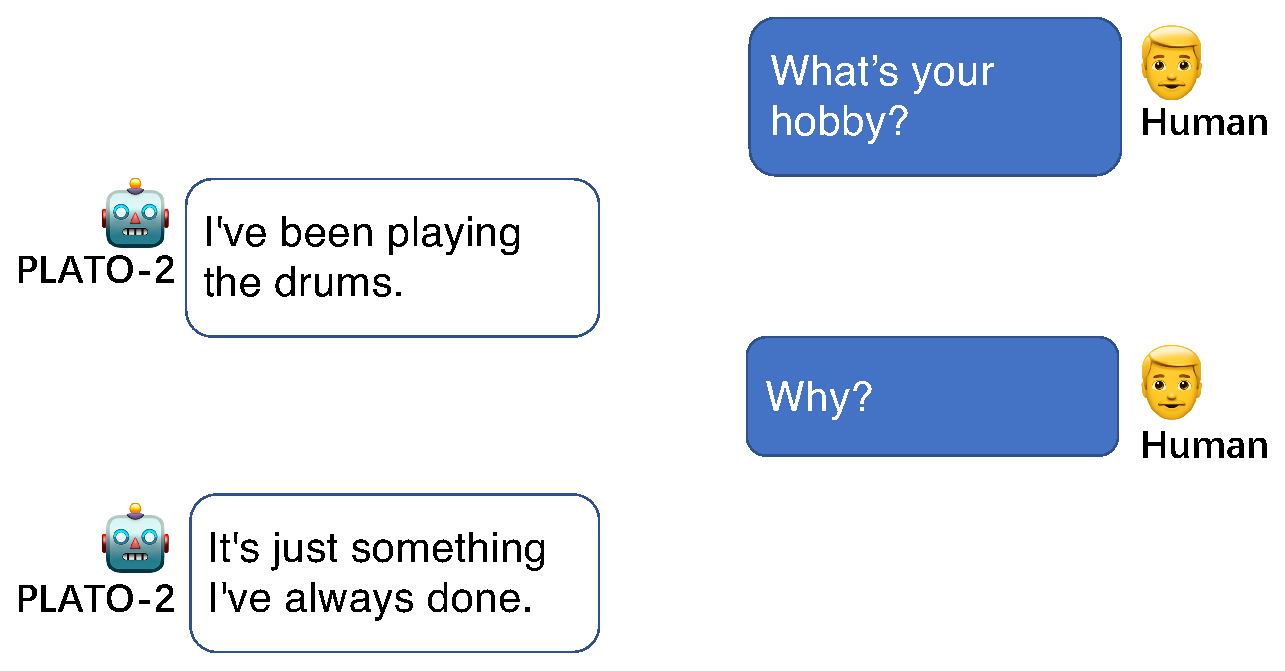
\includegraphics[width=.8\linewidth]{crop1.eps}  
  \caption{A small fragment of conversation between human and bot}
  \label{fig:sub-first}
\end{subfigure}
\begin{subfigure}{0.5\textwidth}
  \centering
  % include second image
  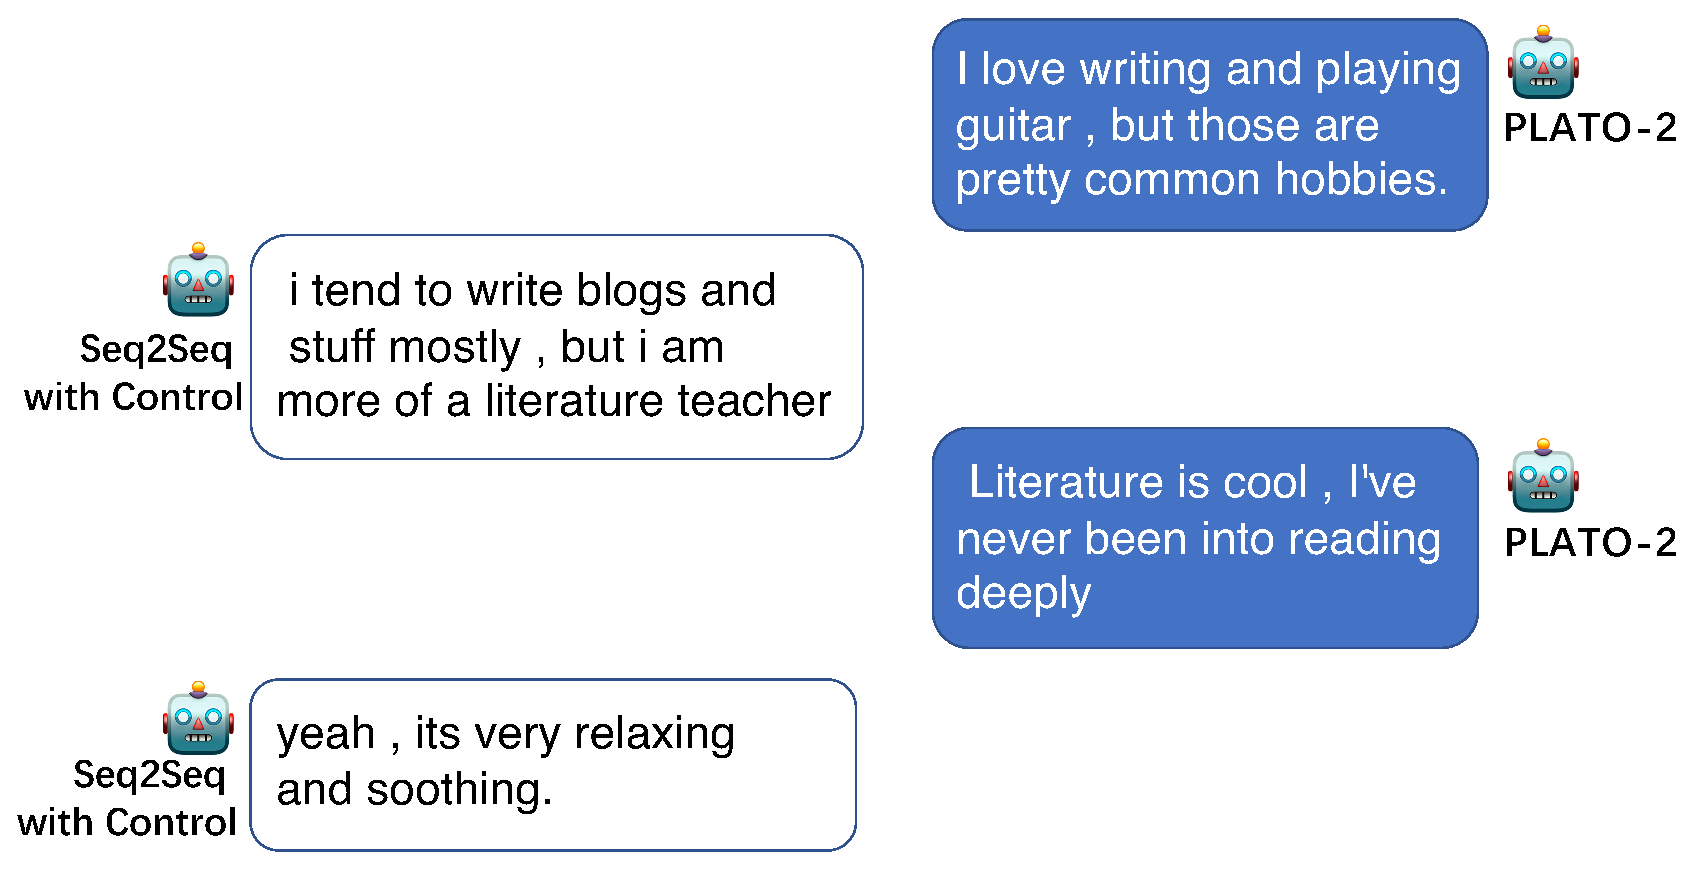
\includegraphics[width=\linewidth]{crop2.eps}  
  \caption{A small fragment of conversation between bot and bot% \KZ{crop the margins
%in this pic or use eps for both.} 
}
  \label{fig:sub-second}
\end{subfigure}
\caption{Small fragments from the chat logs between humans-bot and bot-bot}
\label{fig:two convs}
\end{figure}

Our framework consists of two components: \textit{competition} and 
\textit{scoring}, which may happen simultaneously. The competition is modeled
after most sport tournaments such as soccer or ping pong. 
There are three levels of competitions: 
game-level, match-level and tournament-level. 
Each match consists of several games. During a game, two bots will converse 
freely with each other and a virtual judge will score their performances according to
a group of criteria such as consistency and fluency, etc. 
%As an example like \figref{fig:example} shows, 
%Bot $A$ will be 
%penalized twice for repeating while Bot $B$ will be penalized once for 
%contradicting itself. In addition to the penalty, 
%a bonus point is rewarded to $A$
%who shows to produce relevant response with long term memory. 
%\KZ{Do we still have this as a criterion?}
%However, the specific bonus and penalty settings may vary 
%depending on the domain and scenarios that the experiment is 
%set in. 

%\begin{figure}[th!]
%	\centering
%	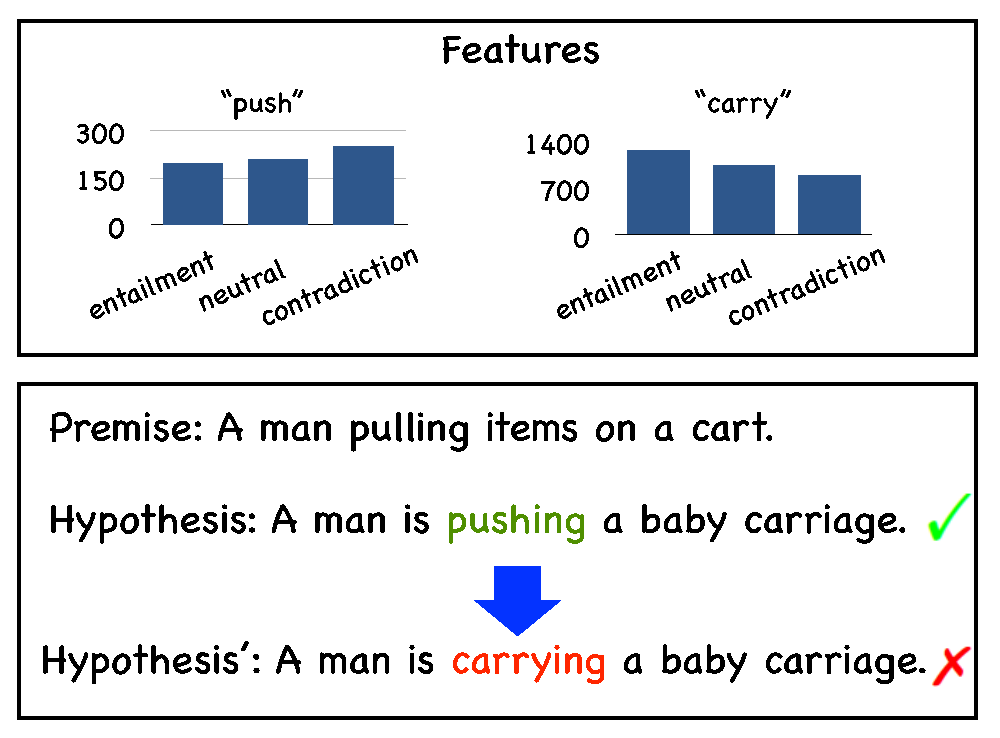
\includegraphics[width=0.95\columnwidth]{example.eps}
%	\caption{A chat snippet between two bots.}
%	\label{fig:example}
%\end{figure}

The main contributions of this paper are:
\begin{itemize}
\item We propose the first interactive evaluation framework for chatbots which
is based solely on bot-to-bot conversations and modeled after sports competitions (\secref{sec:competition}).
\item  The entire scoring process is fully automated and efficient. 
The system can rank seven bots in three minutes on average.
(\secref{sec:scoring}, \secref{sec:time}).
\item  Our experiments show that our scoring system closely tracks the 
human evaluation results. Preliminary results also show
that our evaluation system outperforms 
several recent strong baseline evaluation systems (\secref{sec:main}).
\item %We demonstrate the improvements in efficiency 
%using direct chat logs between bots.
We show that the chats between bots are impressively informative, 
even richer than the chats between humans and bots.
This suggests some possible directions to improve 
the capabilities of bots in the future.
(e.g., by having them learn from each other)  (\secref{sec:diversity})
\end{itemize}

\section{Spatial Features}
\label{chp:spatial}
Considering only one POI's location, it can be as simple as a pair longitude and latitude.
However, with relative position with each other, more information emerges.
Such information is closely related to the POI's functional characteristics,
which indicate their categories. POIs with different categories show different
characteristics on many statistics related to spatial aspects as explained
following in details, and thus different features work well on different
categories. In the following, we analyze different kinds of spatial features
on part of New York data crawled from Foursquare.
We consider only the first level categories for simplicity,
because the same features can be applied to the second level categories
(shown in experiments).

\subsection{Neighborhood Category Distribution}
%\begin{figure}[ht]
%\begin{minipage}{0.5\linewidth}
%\centering
%\includegraphics[width=\columnwidth]{plot/No_other_POI_within_100m.eps}
%\caption{No other POIs within 100m}
%\label{fig:NoPOI}
%\end{minipage}
%\hspace{0.5cm}
%\begin{minipage}{0.5\linewidth}
%\centering
%\includegraphics[width=\columnwidth]{plot/Shop_and_Service_and_Professional_and_Other_Places_neighbor_within_100m.eps}
%\caption{Shop \& Service's and Professional \& Other Places 's neighbor within 100m}
%\label{fig:ShopProf}
%\end{minipage}
%\end{figure}


We observe that POIs related to each other often appear in the same zone.
For example, a shopping center has shops and restaurants, a financial center
has banks and office buildings, or a college town has colleges, museums,
and observatories. Neighborhood shows functionality of an area and thus
provides a prior probability of the category a POI may belong to. In addition,
since different categories show great difference in their neighborhood composition,
neighbourhood profile is also good at differentiating POIs in different categories.

As shown in Figure \ref{fig:NoPOI}, according to our analysis on POIs in New York
from Foursquare data, around 30\% of ``Outdoors \& Recreation'' have no other POIs
near them within 100 meters, indicating their ``isolation'', while most of ``Food'' have
other POIs near them, indicating a symbiotic relationship of ``Food'' with other
interesting spot. The reason is that people often visit a restaurant when 
they are on the way to or leaving some POIs like shops, cinemas, etc.  
%The fact is reasonable since ``Food'' relies on customers visiting,
%however most of restaurants are not attractive enough for people to go there on purpose,
%so they have to bound with places attracting people. \KQ{Don't understand this sentence.
%You mean most of the restaurants are in downtown? should be not attractive enough
%for people to travel a long distance to get there?}
On the contrary, POIs in
``Outdoors \& Recreation'' are usually built in a
large space, thus suburban would be a wise choice. From the figure we can also
see that ``Nightlife Spot'', ``Shop \& Service'' are often around with other POIs,
too, which also gets along with common sense.

Not only the ``crowding'' within a POI's neighborhood differs from one category to another,
the category distribution of the neighborhood also differs from one to another.
Firstly, we should notice that there exists some extreme cases in category
distribution, such as ``Food'' is everywhere while there's very few ``college''
near most of POIs in the city. However, difference still stands out between categories.
As shown in the Figure \ref{fig:ShopProf} we can see there are more food and shops
around ``Shop \& Service'', but there are more ``College \& University'',
``Professional \& Other Places'' near ``College \& University''.
%\begin{figure}[ht]
%\begin{minipage}{0.45\linewidth}
%\centering
%\includegraphics[width=\columnwidth]{plot/F1_measure_using_NB_100_feature.eps}
%\caption{F1 measure using NB\_100m feature}
%\label{fig:F1NB100}
%\end{minipage}
%\begin{minipage}{0.55\linewidth}
%\centering
%\includegraphics[width=\columnwidth]{plot/F1_measure_using_NB_m_feature_on_Shop_and_Service_and_Residence.eps}
%\caption{F1 measure using NB\_m feature on Shop \& Service and Residence with different m}
%\label{fig:F1NBShopResi}
%\end{minipage}
%\end{figure}

Therefore, we introduce NB\_m feature to describe the category distributions
within certain distance around the POI. The NB\_m feature is defined as:
for a POI $i$, the category distribution of all the POIs
within $i$'s m meters and the number of POIs within m meters.

%To prove NB\_m feature's effectiveness, we set $m = 100$ and add NB\_100 feature to BASE feature and test on all categories, it yields better classification result for all as shown in figure \ref{fig:F1NB100}.
%
%Furthermore, with further testing, it appears that different m should be set for different categories. We test on different $m = 10,50,100$, and they result in different performances. Take ``Residence'' and ``Shop \& Service'' as example, as shown in Figure \ref{fig:F1NBShopResi}, NB\_10 yields best result for ``Residence'', and larger m would lower the score, however, ``Shop \& Service'' prefer larger m, and it gains best result when m equals 100.

\begin{figure}
  \centering
  \begin{minipage}[b]{.4\linewidth}
    \centering
    \includegraphics[width=\columnwidth]{plot/No_other_POI_within_100m.eps}
  \end{minipage}%
  %\hspace{-0.75cm}
  \begin{minipage}[b]{.6\linewidth}
    \centering
    %\includegraphics[width=\columnwidth]{plot/Shop_and_Service_and_Professional_and_Other_Places_neighbor_within_100m.eps}
    \includegraphics[width=\columnwidth]{plot/ColorMap/Shop_and_Service_and_Professional_and_Other_Places_neighbor_within_100m.eps}
  \end{minipage}\\%[-10pt]

  \begin{minipage}[t]{.4\linewidth}
    \caption{No other POIs within 100m}
    \label{fig:NoPOI}
  \end{minipage}%
  \hspace{0.3cm}
  \begin{minipage}[t]{.55\linewidth}
    %\caption{Shop \& Service's and Professional \& Other Places 's neighbor within 100m}
    \caption{Different categories'(xtics) category distribution(ytics) within 100m}
    \label{fig:ShopProf}
  \end{minipage}%
\end{figure}

\subsection{ The Nearest K POIs}
%\begin{figure}[ht]
%\begin{minipage}[ht]{0.5\linewidth}
%\centering
%\includegraphics[width=\columnwidth]{plot/Food_and_College_1-Nearest_POI_category_distribution.eps}
%\caption{Food's \& College's 1-Nearest POI category distribution}
%\label{fig:foodcollege}
%\end{minipage}
%\begin{minipage}[ht]{0.5\linewidth}
%\centering
%\includegraphics[width=\columnwidth]{plot/F1_measure_using_N_5_feature.eps}
%\caption{F1 measure using N\_5 feature}
%\label{fig:F1N5}
%\end{minipage}
%\end{figure}


Apart from neighborhood functionality, we find the nearest $k$ POIs'
category as another feature to compensate the NB\_m feature.
It is because the NB\_m feature represents the general
functionality in a big area, but there are often some
concentrations on specific spots. As showed in Figure \ref{fig:foodcollege},
``Food'' and ``College \& University'' show typical intention
aggregating on some spots. For ``College \& University'', no matter
they locate in urban or suburban, the college buildings are definitely
close to each other. And for ``Food'', we can see the trend very often
in our life: there might be a street of local snack, or a part of
business zone full of restaurants. Besides that, other than similar POIs
aggregating together, some categories instinctively near together.
For example, ``Nightlife Spot'' are often mixed with ``Food'',
which is another typical characteristic for both ``Nightlife Spot'' and ``Food''.

It seems that the nearest $k$ POIs feature is a part of POI's neighborhood feature.
However, focusing on the nearest POIs gives extra information on the particular spot the POI is on.
For example, although the neighborhood mainly consists of office buildings,
if the target POI lies in a part of the region that is full of restaurants,
it is more possible that the POI belongs to ``Food''.
In other words, POI's neighborhood is considering a neighborhood based on
the absolute distance, which not only represents the neighborhood's attribute,
but also tells how bustling within the region.
The nearest $k$ POIs feature is a relative neighborhood which considers
only the nearest $k$ POIs, no matter they are far away from each other
or very close to each other. In fact, the two kinds of feature do show
big difference in experiment and we cannot replace one to another.

We use N\_k to abbreviate the nearest k POIs' category distribution.
The N\_k feature is defined as: for a POI i, the category distribution of nearest $k$ POIs within 1km to $i$.

%We further test the influence of selection of k on the result setting $k=1,5,10,20$. According to our experiment, having larger k won't change result very much, we show ``Food'' and ``Nightlife Spot'' as example in Figure \ref{fig:F1NKFoodNight}. However, as we will discuss more in Chapter \ref{Experiment}, since different m in NB\_m will differ very much in result and different m combining different k in N\_k feature will also results in different result, accordingly different k will be needed in final feature construction for different categories.


%{\centering
%\begin{minipage}[ht]{0.5\linewidth}
%\centering
%\includegraphics[width=\columnwidth]{plot/F1_measure_using_N_K_feature_on_Food_and_Nightlife_Spot.eps}
%\captionof{figure}{F1 measure using N\_K feature on Food and Nightlife Spot with different K}
%\label{fig:F1NKFoodNight}
%\end{minipage}
%\begin{minipage}{0.49\linewidth}
%  \centering
%  \small
%  \begin{tabular}{ll}
%
%  \hline\noalign{\smallskip}
%  Category & Distance(m)  \\
%  \noalign{\smallskip}\hline\noalign{\smallskip}
%  Professional \& Other Places  &    210.851 \\
%  Nightlife Spot  &   227.3833 \\
%  Shop \& Service  &   227.5524 \\
%  Arts \& Entertainment  &   230.5648 \\
%  Food  &   237.8074 \\
%  College \& University  &    275.849 \\
%  Residence  &   308.1981 \\
%  \noalign{\smallskip}\hline
%  \end{tabular}
%  \captionof{table}{Different categories' average distance to nearest ``Travel and Transport''}
%  \label{tab:DisToTravel}
%\end{minipage}
%
%}



\begin{figure}[ht]
\centering
%\includegraphics[width=0.7\columnwidth]{plot/Food_and_College_1-Nearest_POI_category_distribution.eps}
\includegraphics[width=0.8\columnwidth]{plot/ColorMap/Food_and_College_1-Nearest_POI_category_distribution.eps}
\caption{Food's \& College's 1-Nearest POI category distribution}
\label{fig:foodcollege}
\end{figure}

\subsection{ Distance to Category}
\label{sec:lcd}
The NB\_m and N\_k feature are insufficient to identify the category for a
POI in some cases. For example, if a POI is located close to a lot of restaurants,
then the POI is supposed to be in category ``Food'' according to the NB\_m and N\_k features.
However, if the POI is far from ``Shop \& Services''
and ``Art \& Entertainments'', then the
POI is probably not a restaurant but a residence.
Due to this fact, we also examine the influence of category
distance, which is the distance from the target POI to
the nearest POI in each category.
%With the NB\_m feature and N\_k feature above, we have a good representation
%for the POIs near the target POI. However, we haven't considered those POIs
%which are not in $m$ meters in NB\_m, and not in the top $k$ list in N\_k.
%There's also a reason why those POIs are, in some sense, far away from the target POI.
%So in order to extract valid information from the POIs that are not near,
%we utilize the feature that shows the distance to the nearest POI in different
%categories, and it exhibits more characteristics. For example, from above
%features including NB\_m and N\_k, a POI shows that it is located close to
%``Food'', based on these, the POI belonging to ``Food'' is a reasonable
%prediction. However, if distance to categories feature tell us more that the
%POI is far from ``Shop \& Services'' and ``Art \& Entertainments'', then the
%probability of the POI belonging to ``Residence'' also rise up.
%We found some interesting facts about category distance.
Specifically, we first examine different categories' average distance
to nearest ``Travel and Transport'' to see which categories are often
near transportation. We show the distances in Table \ref{tab:DisToTravel},
and we find that ``Professional \& Other Places'' is the nearest to transportation,
which is quite reasonable since otherwise the cooperation need to run regular bus for its employees.

\begin{table}[ht]
\centering
%\small
% table caption is above the table
\caption{Different categories' average distance to nearest ��Travel and Transport��}
\label{tab:DisToTravel}       % Give a unique label
% For LaTeX tables use
\begin{tabular}{llll}
\hline\noalign{\smallskip}
Category & Distance(m) &Category & Distance(m) \\
\noalign{\smallskip}\hline\noalign{\smallskip}
Professional \& Other Places  &    \textbf{210.851} &   College \& University  &    275.849   \\
Nightlife Spot  &   227.3833 &Residence  &   308.1981 \\
Shop \& Service  &   227.5524 &Travel \& Transport  & 9788.035\\
Arts \& Entertainment  &   230.5648 &  Outdoors \& Recreation & 12272.19\\
 Food  &   237.8074 & & \\
\noalign{\smallskip}\hline
\end{tabular}
\end{table}

Then, we examine the distance of each category to all other categories in Figure \ref{fig:LogCD}.
From the figure, we observe that ``Outdoor \& Recreation'' is far from all categories,
while ``Food'' is near to all.
This fact gets along with our analysis in Figure \ref{fig:NoPOI} that
there's very few POIs near ``Outdoor'', but ``Food'' can be found everywhere.

Formally, we define the category distance feature ($CD$) for a POI $i$ and a category $c$ as:
\begin{equation}
CD_{i,c}= min_{j \in c} distance(i,j).
\end{equation}

The linear definition of category distance is straightforward but not close to
the fact. POIs in 100km from the target POI and those in 200km
have not much difference for identifying the target POI's category because
both of them are too \emph{far}. In contrast, the classifier should be sensitive
to the difference between two short distances. Therefore, we propose two
variations to $CD$, i.e., $LCD1, LCD2$ as follows:
\begin{align}
LCD1_{i,c} &= \log{(1+CD_{i,c})},\\
LCD2_{i,c} &= \log{(1+\log{(1+CD_{i,c})})}.
\end{align}



%According to our experiment, directly using $CD$ as features in classification is not effective, and a reasonable process is to take log operation, therefore we further define $LCD1, LCD2$ as, for each POI $i$,
%\begin{align}
%LCD1_i &= Log(1+CD_i)\\
%LCD2_i &= Log(1+ Log(1+CD_i))
%\end{align}


%\begin{figure}
%\begin{minipage}[ht]{0.5\linewidth}
%\centering
%\includegraphics[width=\columnwidth]{plot/LogAvgCD.eps}
%\caption{Log(Avg(Category Distance))}
%\label{fig:LogCD}
%\end{minipage}
%\begin{minipage}{0.5\linewidth}
%  %\centering
%  %\raggedleft
%  \includegraphics[width=\columnwidth]{plot/F1_measure_using_LCD1_feature.eps}
%  \caption{F1 measure using LCD1 feature}
%  \label{fig:F1LogCD}
%\end{minipage}
%
%\end{figure}

\begin{figure}[ht]
\centering
\includegraphics[width=0.8\columnwidth]{plot/ColorMap/Color_CategoryDis.eps}
%\caption{Log(Avg(Category Distance))}
\caption{Average Category Distance with log operation, darker indicates a larger distance}
\label{fig:LogCD}
\end{figure}

\subsection{ Region Comparison}


%\begin{figure}[ht]
%\centering
%% Use the relevant command to insert your figure file.
%% For example, with the graphicx package use
%  \epsfig{file=plot/F1_measure_using_RegCom_T_feature.eps,width=0.7\columnwidth}
%% figure caption is below the figure
%\caption{F1 measure using RegCom feature}
%\label{fig:F1RC}       % Give a unique label
%\end{figure}
Region Comparison feature aims at comparing the target POI with other POIs within
the same region on the user behaviors. The motivation is that some categories
may often be ``destinations'' of a user's travel activity, such as ``Art \& Entertainment'',
while some categories may often be on the way to the destination, such as ``Food''.
We assume that the places which are more popular (according to users and check-ins) than other places nearby,
is more probable to be a destination. To make use of the user check-in information,
we consider both the number of check-ins and the number of unique users. We compare
the check-ins and unique users of the target POI to the POIs within a distance of m,
and compute the average difference of check-ins and unique users as the
region comparison feature for the POI. The region comparison feature for total
check-ins (RC\_T\_m(i,c)) and for unique users (RC\_U\_m(i,c)) are computed as follows:
%Thus with such feature, we combine
%the factor from both spatial environment and user behavior. As for user behavior,
%inspired by the previous work, we consider the number of check-ins and unique users.
%Therefore, we compare the target POI's number of total check-ins and unique users
%with the POIs around it, and the region is precisely defined by a radius of m.
%In NB\_m, we apply different m to define neighborhood for different categories,
%likewise, we also build several different Region Comparison features with different m.
%In terms of comparison, we do substraction between the average level of user behavior measures and the target POI's digits. Formally, we define $Region Comparison\_Total Check-in (RC\_T\_m)$ and $Region Comparison\_Unique Users (RC\_U\_m)$ as
\begin{equation}
RC\_T\_m(i,c) = Avg_{j \in c, distance(i,j)<m} \#Checkin(j) - \#Checkin(i) 
\label{eq:rct}
\end{equation}
\begin{equation}
RC\_U\_m(i,c) = Avg_{j \in c, distance(i,j)<m} \#UniqueUser(j) - \#UniqueUser(i)
\label{eq:rcu}
\end{equation}

Figure \ref{fig:RC} shows the average region comparison feature of 
total check-ins for the five categories of POIs.
The score below 0 means that people check in more times at target POI than the POIs near it.
%Checking in a place more than the ones near it is actually saying that people are gathered to the place, or in other word, it is a ``destination'', not a ``by the way''.
Intuitively, ``Art \& Entertainment'' is more of a ``destination'', people come in purpose
to watch a show, or see an exhibition. ``Outdoor \& Recreation'' is more of a ``destination'', too,
since people planned beforehand to have a weekend with children on a beach, or have a routine of
going to fishing spot. ``Food'' is a ``on the way'' category both by intuition and statistics.
People grab something to eat all the time: after a walk or before a movie. Interestingly, we
find that ``Shop \& Service'' shows the character of a ``by the way'', too.
It seems interesting shops are growing in number, and consequently people are attracted into a
shop though not intended. In contrast, nightlife spot's are more of destinations, because they 
are usually the last places people may visit in daily life. 
%it seems bars are getting more popularity and loyalty from customers than shops and food.

%To show the strength of region comparison features, we set m to be 100 for both RC\_T\_m and RC\_U\_m, and test the features on the nine first level categories, the result is shown in Figure \ref{fig:F1RC}. When the features are combining with BASE and m set to be 100, RC\_T\_m and RC\_U\_m show similar strength in classification, however, as we will discuss more on experiment in Chapter \ref{Experiment}, RC\_U\_m appears to be more effective than RC\_T\_m. Overall, they do show improvements but not as powerful as previous ones.
\begin{figure}[ht]
% Use the relevant command to insert your figure file.
% For example, with the graphicx package use
  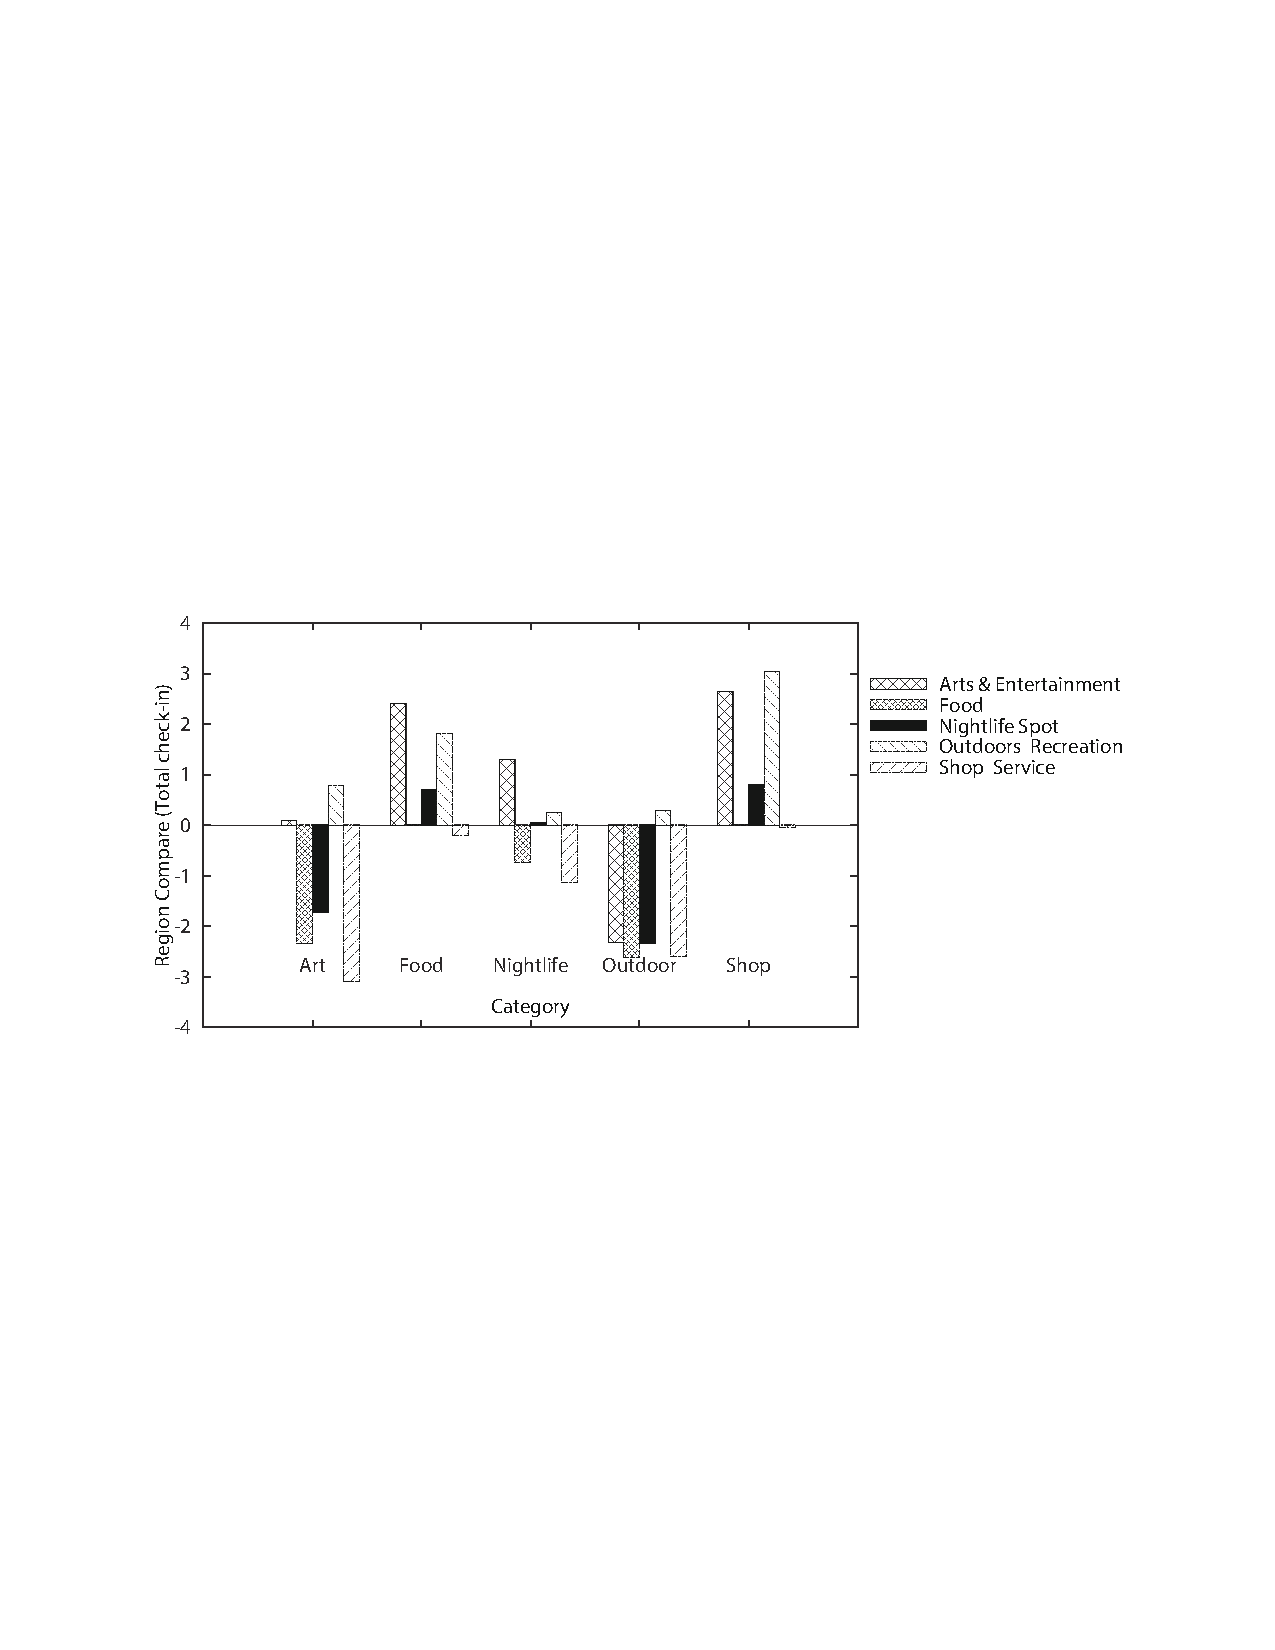
\epsfig{file=plot/RegionCompare.pdf,width=\columnwidth}
% figure caption is below the figure
\caption{Region Compare (Total Check-ins), score below 0 indicates more check-in time than other categories within same region}
\label{fig:RC}       % Give a unique label
\end{figure}

\section{Other Features}
\label{chp:others}
\subsection{NAME Features}
The most direct way to discover the category of a POI is looking at its name.
%Similar with human guessing the category of a POI, the first intuition we get from a POI is its name.
For example, when we see a POI named ``Mouth Restaurant'', we would easily figure out that it belongs to ``Food''.
%Given the fact that words appear in POIs' names are far more less than in vocabulary,
We build the NAME feature in a straightforward way. We break POIs' names into words,
then we collect all the words and filter out those showed up only once in POIs.
Then the remaining words forms a dictionary, and NAME feature for a POI is the
binary representation of the POI's name in the dictionary.

Simple as it is, it is obvious that NAME feature is a powerful feature.
However, there's still cases that name features cannot help but other features work.
For example, when we meet the name ``Charlie's Corner'', it is not so obvious what category
it should belong to by looking at the name. However, it shows good visit time distribution,
as well as good spatial environment character with other ``Food'' near it,
thus we still can classify it to ``Food'', which is the correct label, over other categories.

\subsection{BASE Features}
\label{sec:base}
As discussed above, the statistics of user behavior
features in Ye et al.'s work \cite{yemao} are also effective features for identifying
a POI's category. We also employ these feature in our experiments.
These features include the total number of check-ins, unique visitors,
maximum number of check-ins by a single visitor, distribution of check-in
time in a week and in 24-hour scale. %Such features represent the user behavior very well.



\section{Evaluation}
\label{sec:evaluation}
Through the above approach, we translate two popular English knowledge graphs: \con and \pro into \zhcon and \zhpro, respectively. In terms of the word embedding, we use the Chinese Wikipedia dump on Aug 1, 2018,  to train word embedding with Word2Vec, where the vocabulary size is 110,978 and the embedding dimension is 300.\footnote{\url{https://code.google.com/archive/p/word2vec/}}
In this section, we evaluate the coverage and accuracy of \zhcon and \zhpro, respectively. The baseline experiment we choose is the direct translation using the translator, and we will denote it as \textbf{DT} later. For example, in the baseline, we translate triple (``ball'', AtLocation, ``ballroom'') by feeding ``ball, ballroom'' into translator, and split the translation result ``球, 舞厅'' into (``球'', AtLocation, ``舞厅'') as the final translation result. Here, we do not provide the translator with the contextualized sentence such as ``the ball is at the ballroom.'', since there are no fixed patterns in the translated sentence, which makes it hard to extract the corresponding part, even for the translated results of one particular relation.\footnote{For example, although ``french chefs are capable of preparing food.'' and ``spider web is capable of catching morning dew.'' share the same structure in English, they will be translated into ``法国厨师有能力准备食物。'' and ``蜘蛛网能够吸引晨露。'' respectively, which requires more than one pattern to split the translation result.}

%\KZ{In addition to the end-to-end eval on the two translated KBs, you also
%need to do some ablation tests. For example, what if you don't do the revision?
%Is there any alternative ways to do revision? You need to show that your way of
%revision is better than straightforward methods.}

\subsection{\zhcon}
\zhcon is a mixed Chinese common sense knowledge graph, which comes from two sources, 
the original Chinese part of \con and the translation result of the English part of \con.

\textbf{Coverage.}
As shown in Table \ref{tab:zh_conceptnet_coverage}, the size of \zhcon is \textbf{4.76} times as large as the original Chinese part of \con, 
which is a substantial increase in quantity. The size of \zhpro is not as 4.91 times as we expected, since there exists overlap in the process of merging.
To our best knowledge, there are no other Chinese knowledge graphs dedicated to common sense, and \zhcon will be the first large one with about 2 million edges, which, we hope, could be a valuable asset for Chinese common sense research.
\begin{table}[ht]
\caption{Size of \zhcon.}
\label{tab:zh_conceptnet_coverage}
\centering
\begin{tabular}{ll}\hline 
\textbf{Dataset}&\textbf{Size}\\\hline
1. Original Chinese Part in \con &438,307(x1.00)\\  
2. Translated English part in \con &1,716,327(x3.91)\\
\zhcon (Merge 1 and 2)&\textbf{2,085,681(x4.76}) \\\hline
\end{tabular}
\end{table}

\textbf{Accuracy.}
To evaluate the quality of \zhcon, 
we randomly sample 500 samples from original Chinese part in \con, 
\text{DT} result of English part in \con, translation result of English part in \con based on our two-steps approach (we denote it as \textbf{OURS} later), and \zhcon (which merges the Chinese part in \con and translated English part in \con of \textbf{OURS}), respectively. 
We ask two annotators to evaluate these samples. 
As Table \ref{tab:conceptnet_accuracy} shows, there exists 1\% error in the original Chinese part of \con, which comes from crowdsourcing errors.
%Since approximately 86\% of the data in \con comes from collaborative datasets, such as Wiktionary, DBpedia, etc 
Compared with the direct translation (\text{DT}), the accuracy of the translation result based on \textbf{OURS} has a relative gain of \textbf{2.8\%}.
The accuracy of \zhcon has also been improved to \textbf{89.6\%} due to the high quality of the merged original Chinese part from \con.

\begin{table}[ht]
\caption{Accuracy of different approaches. The Kappa coefficients \cite{landis1977measurement} of two annotators suggest a substantial agreement.}
\label{tab:conceptnet_accuracy}
\centering
\begin{tabular}{ll}\hline
	Approach & Accuracy (Kappa) \\ \hline
	1. Original Chinese part in Conceptnet& 98.3\%(0.58) \\
	2. \textbf{DT} of English part                 & 84.5\%(0.85) \\
	3. \textbf{OURS} & 87.3\%(0.85) \\
	Zh-Conceptnet (Merge 1 and 3) & \textbf{89.6\%(0.79)} \\\hline
\end{tabular}
\end{table}

\textbf{Qualitative Results.}
Our approach can handle some intractable word sense disambiguations, such as ``date'', ``ball'', ``court'', ``capital'', ``fan'', etc, as shown in the blue part in Table \ref{tab:zh_conceptnet_case}.
Besides, our method can translate (``fan'', RelatedTo, ``sector'') into (``扇'', RelatedTo, ``扇形''), while the result of \textbf{DT} is (``粉丝'', RelatedTo, ``部门''). This shows that our approach can disambiguate ``fan''  and ``sector'' at the same time. As for the errors in \zhcon, according to our observations, most errors in \zhcon come from the triples with the relation of ``RelatedTo''. Since the relation of ``RelatedTo'' is relatively weak in English such as (``blunt'', RelatedTo, ``money''), it becomes even weaker after translation, and the triples with the relation of ``RelatedTo'' account for 48.16\% of all the triples in \con. The red part in Table \ref{tab:zh_conceptnet_case} shows more error cases. 


\begin{table}[!htbp]
\caption{Some examples triples in \zhcon. Correct translations are in {\color{blue} blue}, and incorrect ones are in {\color{red}red}.}
\label{tab:zh_conceptnet_case}
\resizebox{\linewidth}{!}{%
\begin{tabular}{lll}\hline
	\textbf{English}                 & \textbf{OURS}     & \textbf{DT}  \\\hline
	{\color{blue}(date, fruit)/IsA}                  & {\color{blue}枣, 水果}     & {\color{blue}时间, 水果}    \\ 
	{\color{blue}(ball, ballroom)/AtLocation}        & {\color{blue}舞会, 舞厅}    & {\color{blue}球, 舞厅}     \\ 
	{\color{blue}(can, shelf)/AtLocation}            & {\color{blue}罐头, 货架}    & {\color{blue}可以, 货架}    \\ 
	{\color{blue}(court, gymnasium)/AtLocation}       & {\color{blue}球场, 体育馆}   & {\color{blue}法院, 体育馆}   \\ 
	{\color{blue}(munition, arm)/MannerOf}            & {\color{blue}军火, 武装}    & {\color{blue}军火, 手臂}    \\ 
	{\color{blue}(capital, proper noun)/AtLocation} & {\color{blue}大写, 专有名词}  & {\color{blue}资本, 专有名词}  \\ 
	{\color{blue}(spinach, can)/RelatedTo}             & {\color{blue}菠菜, 罐头}    & {\color{blue}菠菜, 可以}    \\ 
	{\color{blue}(fan, blow)/RelatedTo}             & {\color{blue}扇子, 吹}    & {\color{blue}粉丝, 吹}    \\ 
	{\color{blue}(fan, peacock)/RelatedTo}             & {\color{blue}扇子, 孔雀}    & {\color{blue}粉丝, 孔雀}    \\ 
	{\color{blue}(fan, sector)/RelatedTo}             & {\color{blue}扇, 扇形}    & {\color{blue}粉丝, 部门}    \\ 
	{\color{blue}(collection, garage)/AtLocation}             & {\color{blue}珍藏, 车库}    & {\color{blue}集合, 车库}    \\ 
	{\color{blue}(brook, tolerate)/RelatedTo}             & {\color{blue}容忍, 姑息}    & {\color{blue}小溪, 容忍}    \\ 
	{\color{red} (blunt, money)/RelatedTo}             & {\color{red} 生硬, 钱}    & {\color{red} 生硬, 钱}    \\ 
	{\color{red} (fouta, thin)/RelatedTo}             & {\color{red}伏塔加, 瘦}    & {\color{red}富塔, 瘦}    \\ 
	{\color{red}(major ninth, interval)/RelatedTo}             & {\color{red}主要的第九, 间隙}    & {\color{red}主要的第九, 间隔}    \\ 
	{\color{red}(melo, music)/RelatedTo}             & {\color{red}甜瓜, 音乐}    & {\color{red}melo, 音乐}    \\ \hline
\end{tabular}}
\end{table}

%粉丝    /r/RelatedTo    打击
%fan     ['球迷', '迷', '风扇', '扇子', '扇', '粉丝']
%blow    ['打击', '吹', '刮']
%扇子    吹      0.29190982571468305
%(fan, blow)/RelatedTo             & 扇子, 吹    & 粉丝, 吹    \\ \hline
%
%粉丝    /r/RelatedTo    孔雀
%fan     ['球迷', '迷', '风扇', '扇子', '扇', '粉丝']
%peacock ['孔雀']
%扇子    孔雀    0.2387474142191117
%(fan, peacock)/RelatedTo             & 扇子, 孔雀    & 粉丝, 孔雀    \\ \hline
%
%粉丝    /r/RelatedTo    部门
%fan     ['球迷', '迷', '风扇', '扇子', '扇', '粉丝']
%sector  ['扇形', '部门']
%扇      扇形    0.2658884528019793
%(fan,sector)/RelatedTo             & 扇, 扇形    & 粉丝, 部门    \\ \hline
% 
%\begin{table}[th]
%\caption{Some examples triples in \zhcon}
%\label{tab:conceptnet_case}
%\center
%\begin{tabular}{|l|l|l|}\hline
%\textbf{Node1(Subject)} & \textbf{Relation} & \textbf{Node2(Object)} \\ \hline\hline
%	\begin{tabular}[c]{@{}l@{}}植物/plant\end{tabular} & /r/Desires & 水和太阳/water\_and\_sun \\ \hline
%	\begin{tabular}[c]{@{}l@{}}植物/plant\end{tabular} & /r/AtLocation & \begin{tabular}[c]{@{}l@{}}污垢/dirt,\\花盆/flower\_pot,\\花园/garden\end{tabular} \\ \hline
%	
%	\begin{tabular}[c]{@{}l@{}}植物/plant\end{tabular} & /r/Antonym & \begin{tabular}[c]{@{}l@{}}矿物/mineral,\\动物/animal\end{tabular}\\ \hline
%	
%	\begin{tabular}[c]{@{}l@{}}植物/plant\end{tabular} & /r/NotCapableOf & \begin{tabular}[c]{@{}l@{}}移动/move,\\跑/run,\\想想/think,\\走路/walk\end{tabular} \\ \hline
%	
%	\begin{tabular}[c]{@{}l@{}}工厂/plant\end{tabular} & /r/RelatedTo & \begin{tabular}[c]{@{}l@{}}设施/facility,\\制造业/manufacturing,\\起动器/starter\\机械/machinery\end{tabular} \\ \hline
%	%					工厂(factory)\\/plant & /r/IsA & \begin{tabular}[c]{@{}l@{}}包装厂/packinghouse,回收厂/recycling\_plant,\\ 炼油厂/refinery\end{tabular} \\ \hline
%	\begin{tabular}[c]{@{}l@{}}植物/plant\end{tabular} & /r/CapableOf & \begin{tabular}[c]{@{}l@{}}绽放/bloom,\\成长/grow,\\光合作用/photosynthesis\end{tabular}  \\\hline
%\end{tabular}
%\end{table}

\subsection{\zhpro}
We translate \pro into \zhpro based on our proposed approach. In this section, we compare \zhpro with two well-known Chinese taxonomic knowledge graphs CN-Probase \cite{Xu2017} and zhishi.me \cite{Niu2011} in terms of coverage and accuracy.

\textbf{Coverage.}
As shown in Table \ref{tab:zh_probase_coverage}, \zhpro has the same order of magnitude as CN-Probase and is \textbf{11.74} times larger than zhishi.me. 
We further evaluate the overlap between \zhpro and existing Chinese taxonomic knowledge graphs.
Since CN-Probase is not open-source, to calculate the ratio of overlap, we apply the method of sampling. First, we sample 500 ``IsA'' pairs from CN-Probase via the public API of CN-Probase and count the ratio of overlap with \zhpro, which is only \textbf{1\%}. Then, we sample 500 ``IsA'' pairs from \zhpro, and get the ratio of \textbf{6\%}. The intersection of \zhpro and zhishi.me is only \textbf{5,243} pairs.
The reasons why the overlap ratio between \zhpro and CN-Probase is small are as follows: First, as shown in Table \ref{tab:zh_probase_coverage}, CN-Probase has more instances and fewer concepts, like the shape of the Pyramid, while \zhpro has more concepts and fewer instances, like the shape of the inverted Pyramid. 
Second, most entities in \zhpro are translated from English, which only exist in English context, while entities in CN-Probase are extracted from the high-quality Chinese encyclopedia. The third reason is that many latest entities are collected in CN-Probase, while not in \zhpro, since the publish time of CN-Probase is later.
Due to the small overlap between \zhpro and existing Chinese taxonomic knowledge graphs, \zhpro can substantially enrich them. Also, due to the large concept space and broader topics, it will exhibit a stronger ability in capturing the implied semantics, as demonstrated in \cite{wang2010toward}.
Therefore, we can conclude that although the number of ``IsA" pairs in CN-Probase is 3 times larger than that in \zhpro, \zhpro can still greatly enrich existing Chinese taxonomic knowledge graphs.

%The ratio of pairs in CN-Probase, which are also in \zhpro, is \textbf{6\%}, while the ratio of ``IsA'' pairs in \zhpro, which are also in CN-Probase, is less than \textbf{1\%}. This is the sampling estimate via the public API interface of CN-Probase, since it is not open-source.
%The size of the concepts in \zhpro (2,094,825) is \textbf{8} times larger than that in CN-Probase (270,000) while the number of the instances of \zhpro (4,532,110) is much less than CN-Probase (17,000,000). The reason may be that the data sources of both CN-Probase and zhishi.me come from Baidu Baike, Hudong Baike and Chinese Wikipedia (three largest Chinese encyclopedia websites), which, more specifically, come from the well-formed information, such as abstract, infobox, category information, therefore, the instance space of these two knowledge graphs is extremely large while the concept space is relatively small. 
%For example, in CN-Probase, the top instances of concept ``人/person'' are always specific person names, such as ``曹操'', ``崔健'', ``李清云'', etc.
%In contrast, the data source of \pro is massive text corpora in online webpages, which is freer than the data source of CN-Probase, thus, its concept space is large.
%For example, the top instances of concept ``人/person'' in \zhpro are all sub-concepts, such as ``老人/old people'', ``朋友/friend'', ``医生/doctor'', etc.


%\KZ{The style and font size of all tables must be consistent. You can't use 
%resizebox to scale everything into one column so that the fontsizes are
%different.}
\begin{table}[ht]
\caption{Size of existing taxonomic knowledge graphs. (`-' means we cannot get it. ``con-ins'' means ``concept-instance''. ``con-subc'' means ``concept-subconcept''.)}
\label{tab:zh_probase_coverage}
\centering
\begin{tabular}{cccc}\hline
	\textbf{}&\textbf{\zhpro}&\textbf{CN-Probase}&\textbf{zhishi.me}\\ \hline
	concepts  &\textbf{2,094,825}&270,000&17,936\\
	instances  &4,532,110&17,000,000&511,667\\
	con-ins pairs &\textbf{7,054,382}&-&959,581\\
	con-subc pairs&\textbf{4,238,111}&-&2,003\\
	IsA pairs&11,292,493&33,000,000&961,587 \\ \hline
	\end{tabular}
\end{table}

\textbf{Accuracy.}	
To evaluate the quality of \zhpro, 
we randomly sample 500 samples from \pro, \textbf{DT} result of \pro, translation result based on \textbf{OURS}, respectively.
We ask two annotators to evaluate these samples. 
The results are shown in Table \ref{tab:probase_accuracy}. 
Compared with \textbf{DT}, the accuracy based on \textbf{OURS} has increased by \textbf{1.4\%} (from 85.2\% to 86.6\%).
It is less than the improvement (2.8\%) of translation result based on \textbf{OURS} in
\zhcon, because most nodes in \pro are less ambiguous multi-words.
In addition to the inherent error around 7\% (accuracy 93.0\%) in \pro, our translation approach only introduces an additional error of 6.4\% (accuracy 86.6\%), which will be analyzed in the next section. 
\begin{table}[ht]
\caption{The accuracy of existing Chinese taxonomic graphs. The Kappa coefficients of two annotators suggest the substantial agreement.  }
\label{tab:probase_accuracy}
\centering
\begin{tabular}{ll}\hline
	\textbf{Knowledge Graph} & \textbf{Accuracy(Kappa)} \\ \hline 
	\pro    & 93.0\%(0.75) \\ 
	\textbf{DT} of \pro    & 85.2\%(0.84) \\ 
	Zh-Probase & 86.6\%(0.88) \\ 
	CN-Probase     & 95.0\% \\ 
	zhishi.me     & 100\% \\ \hline
\end{tabular}
\end{table}

\textbf{Qualitative Results.}
Our approach can handle some intractable word sense disambiguations, such as ``bank'', ``bark'', ``scale'' etc, as shown in the blue part in Table \ref{tab:probase_case}. On the other hand, there also exist some errors introduced by our method. 
Typical error cases are shown in the red part in Table \ref{tab:probase_case}. According to our observation, most of the errors come from two sources. 
First, translating the entities directly leads to ambiguous Chinese results.
For example, (``go move shift'', IsA, ``song'') will be translated into (``去转移'', IsA, ``歌曲''), which is hard to understand in Chinese. However, translation of named entities is hard to be avoided because not all the first letter of named entities will be capitalized.
Second, the machine translator sometimes cannot return all the Chinese word senses of the word. For example, (``florist'', isA, ``outlet'') will be incorrectly translated into (``花商'', isA, ``出口'') because the translator does not return the Chinese word sense ``批发商店'', which is the correct Chinese word sense of ``outlet'' here.

\begin{table}[!htbp]
	\caption{Some ``IsA'' samples in \zhpro. Correct translations are in {\color{blue} blue}, and incorrect ones are in {\color{red}red}.}
	\label{tab:probase_case}
	\resizebox{\linewidth}{!}{%
		\begin{tabular}{lll}\hline
			\textbf{English}                            & \textbf{OURS}     & \textbf{DT} \\\hline
			{\color{blue} (bank, natural feature)}          & {\color{blue}岸边, 自然特征} & {\color{blue}银行, 自然特征} \\
			{\color{blue}(bank, man-made boundary)}        &  {\color{blue}岸边, 人造边界}  & {\color{blue}银行, 人造边界}  \\
			{\color{blue}(grand Arab capital, capital)}    & {\color{blue}阿拉伯首都, 首都} & {\color{blue}阿拉伯首都, 资本} \\
			{\color{blue}(spring, natural water)}          & {\color{blue}泉水, 天然水}   &  {\color{blue}春天, 天然水}   \\
			{\color{blue}(spring, surface water)}          & {\color{blue}泉水, 地表水}   &  {\color{blue}春天, 地表水}   \\
			{\color{blue}(bark, close range vocalization)}&{\color{blue}吠,近距离发声}&{\color{blue}树皮,近距离发声}\\
			{\color{blue}(bark, vocalization)}&{\color{blue}吠,发声}&{\color{blue}树皮,发声}\\
			{\color{blue}(scale, graphic learning material)}&{\color{blue}比例尺, 图形学习材料}&{\color{blue}规模, 图形学习材料}\\
			{\color{blue}(scale, voice exercise)}&{\color{blue}音阶, 语音练习}&{\color{blue}规模, 语音练习}\\
			{\color{blue}(scale, animal covering)}&{\color{blue}鳞, 动物覆盖}&{\color{blue}规模, 动物覆盖}\\
			{\color{blue}(scale, musicianship skill)}&{\color{blue}音阶, 音乐技巧}&{\color{blue}规模, 音乐技巧}\\
			{\color{blue}(ball, social event)}&{\color{blue}舞会, 社交活动}&{\color{blue}球, 社交活动}\\
			{\color{blue}(ball, physical activity)}&{\color{blue}舞会, 体力活动}&{\color{blue}球, 身体活动}\\
			{\color{blue}(ball, celebration)}&{\color{blue}舞会, 庆祝}&{\color{blue}球, 庆祝}\\
			{\color{blue}(fan, artifact)}&{\color{blue}扇子, 人工制品}&{\color{blue}粉丝, 人工制品}\\
			{\color{red}(florist, outlet)}&{\color{red}花商, 出口}&{\color{red}花店, 出口}\\
			{\color{red}(go move shift, song)}&{\color{red}去移动, 鸣声}&{\color{red}转移, 歌曲}\\
			{\color{red}(Banks of the Ohio, song)}&{\color{red}俄亥俄州的银行, 曲子}&{\color{red}俄亥俄州的银行, 歌}\\
			{\color{red}(chin check, song)}&{\color{red}下巴检查, 鸣声}&{\color{red}下巴检查, 歌}\\\hline
		\end{tabular}
	}
\end{table}

%\subsection{Discussion of First step of \textbf{OURS}}
%%probase 22 16
%%probase 26 12  4770716/11292493=0.422
%total error:
%probase 11\%,13\%    ave:12\%
%
%-inner error
%probase 3\%, 7\%    ave:5\%
%
%%%%%%%%conceptnet 200 43 11  241962/2085681=0.116
%
%%conceptnet 200 15  3
%%conceptnet 200 28 9  241962/2085681=0.116
%total error:
%conceptnet 7.5\%,14\%  ave:10.75\%
%-inner error
%conceptnet 6\%, 9.5\%  ave:7.75\%
%
%hj:
%conceptnet 2,3,4:19,3,8
%probase 2,3,4: 22,16,7
%xr:
%conceptnet 2,3,4:27,9,12
%probase 2,3,4: 22,8,9
%
%
%wsd:
%conceptnet  5.5\%,7.5\% ave: 6.5\%
%probase: 7.5\%,6.5\% ave:7\%


%\begin{table}[H]
%\caption{Some ``IsA'' samples in \zhpro}
%\label{tab:probase_case}
%\begin{tabular}{|l|l|l|}
%	\hline
%	\textbf{Instance} & \textbf{Subconcept} & \textbf{Concept} \\ \hline\hline
%	\begin{tabular}[c]{@{}l@{}}番茄(tomato)\\玉米(maize, corn)\\大豆(soy, soybean)\end{tabular} & 
%	\begin{tabular}[c]{@{}l@{}}植物\\(plant, flora)\end{tabular} &
%	\begin{tabular}[c]{@{}l@{}}有机体(organism)\\ 生产者(producer)\end{tabular} \\ \hline
%	
%	%		\begin{tabular}[c]{@{}l@{}}无水乙醇/(anhydrous ethyl alcohol)\\ 合成乙醇/(synthetic ethyl alcohol)\end{tabular} & 
%	%		\begin{tabular}[c]{@{}l@{}}乙醇\\(alcohol,ethanol)\end{tabular}&
%	%	    \begin{tabular}[c]{@{}l@{}}生物燃料/(biological fuel)\\ 有机溶剂/(organic solvent)\\ 化合物/(compound)\end{tabular} \\ \hline
%	
%	\begin{tabular}[c]{@{}l@{}}橡胶厂(rubber plant)\\
%		炼油厂(oil refinery)\\ 电厂(power plant)\end{tabular} & \begin{tabular}[c]{@{}l@{}}工厂\\(factory, mill)\end{tabular} & \begin{tabular}[c]{@{}l@{}}资产(asset)\\地方(spot,place)\end{tabular} \\ \hline
%	
%	\begin{tabular}[c]{@{}l@{}}狗(dog),猫(cat,feline)\\ 牛(cattle,cow,ox)\end{tabular} &
%	\begin{tabular}[c]{@{}l@{}} 动物\\(animal)\end{tabular} & \begin{tabular}[c]{@{}l@{}}类别(category)\\
%		主题(theme)\\ 
%		生物(creature)\end{tabular}\\ \hline
%\end{tabular}
%\end{table}

%
%近距离发声      IsA     树皮
%close range vocalization        ['近距离发声']
%bark    ['吠', '树皮']
%近距离发声      吠      0.22152851973712392
%近距离发声      树皮    0.07381855955982522
%(bark, close range vocalization)&吠,近距离发声&树皮,近距离发声\\\hline
%
%发声    IsA     树皮
%vocalization    ['发声']
%bark    ['吠', '树皮']
%发声    吠      0.20266486701662512
%发声    树皮    0.02289122701292446
%(bark, vocalization)&吠,发声&树皮,发声\\\hline
%
%图形学习材料    IsA     规模
%graphic learning material       ['图形学习资料', '图形学习材料']
%scale   ['音阶', '规模', '级别', '尺度', '鳞', '比例', '比例尺']
%图形学习材料    比例尺  0.268557394974322
%图形学习材料    尺度    0.21657940353240107
%(scale, graphic learning material)&比例尺, 图形学习材料&规模, 图形学习材料\\\hline
%
%语音练习        IsA     规模
%voice exercise  ['配音练习', '语音练习']
%scale   ['音阶', '规模', '级别', '尺度', '鳞', '比例', '比例尺']
%语音练习        音阶    0.31595054519851007
%(scale, voice exercise)&音阶, 语音练习&规模, 语音练习\\\hline
%
%动物覆盖        IsA     规模
%animal covering ['动物覆盖物', '动物覆盖']
%scale   ['音阶', '规模', '级别', '尺度', '鳞', '比例', '比例尺']
%动物覆盖        鳞      0.2980978974505864
%动物覆盖        尺度    0.2653591599617439
%(scale, animal covering)&鳞, 动物覆盖&规模, 动物覆盖\\\hline
%
%音乐技巧        IsA     规模
%musicianship skill      ['音乐才能', '音乐技巧']
%scale   ['音阶', '规模', '级别', '尺度', '鳞', '比例', '比例尺']
%音乐技巧        音阶    0.3543777738132791
%(scale, musicianship skill)&音阶, 音乐技巧&规模, 音乐技巧\\\hline
%
%社交活动        IsA     球
%social event    ['社交活动']
%ball    ['球', '舞会', '丸子']
%社交活动        舞会    0.5062901630643256
%(ball, social event)&舞会, 社交活动&球, 社交活动\\\hline
%
%身体活动        IsA     球
%physical activity       ['体力活动', '身体活动']
%ball    ['球', '舞会', '丸子']
%身体活动        舞会    0.30998053650136403
%体力活动        舞会    0.2693407790252701
%(ball, physical activity)&舞会, 体力活动&球, 身体活动\\\hline
%
%庆祝    IsA     球
%celebration     ['庆典', '典礼', '庆祝']
%ball    ['球', '舞会', '丸子']
%庆典    舞会    0.5391221765807583
%(ball, celebration)&舞会, 庆祝&球, 庆祝\\\hline
%
%每日文章        IsA     粉丝
%everyday article        ['日常用品', '每日文章']
%fan     ['扇子', '爱好者', '球迷', '风扇', '迷', '粉丝']
%日常用品        扇子    0.24773631914892047
%每日文章        爱好者  0.19835457168625464
%(fan, everyday article)&扇子, 日常用品&粉丝, 每日文章\\\hline
%
%人工制品        IsA     粉丝
%artefact        ['假象', '人工制品']
%fan     ['扇子', '爱好者', '球迷', '风扇', '迷', '粉丝']
%人工制品        扇子    0.09307627931322751
%(fan, artefact)&扇子, 人工制品&粉丝, 人工制品\\\hline

\section{Related Work}
%Ruolan should write this part.
Early work on rewriting often considers the problem as a 
standard text generation task,
using pointer networks 
or sequence-to-sequence models %\citep{elgohary-etal-2019-unpack,quan-etal-2019-gecor} 
with a copy mechanism 
\citep{su-etal-2019-improving,elgohary-etal-2019-unpack,quan-etal-2019-gecor}
to fetch the relevant information in the context \citep{gu-etal-2016-incorporating}.
Later, pre-trained model like T5 \citep{2020t5} are fine-tuned with conversational 
query reformulation dataset to generate the rewritten utterance directly. \citet{DBLP:journals/corr/abs-2204-03958} uses Picker which identifies the omitted tokens to optimize T5. We the results in their paper, 
therefore, we did not compare with it in the experiments. In general, these generative approaches ignore the characteristic of IUR problem: rewritten utterances often share the same syntactic structure as the original incomplete utterances.

Given that coreference is a major 
source of incompleteness of an utterance,
another common thought is to utilize a 
coreference resolution or corresponding 
feartures. 
\citet{tseng-etal-2021-cread} 
proposed a model which jointly learns coreference resolution
and query rewrite 
with the GPT-2 architecture \citep{Radford2019LanguageMA}.
By first predicting coreference links
between the query and context,
the performance of rewriting has improved 
while the incompleteness is induced
by coreference.
However, this does not work for utterances
with ellipisis. Besides, the performance of 
the rewriting
 model is limited by
the coreference resolution model.

Recently, some of the work on 
incomplete utterance rewriting 
focuses on the ``actions'' we
take to change the original
incomplete utterance
into a self-contained
utterance (target utterance).
\citet{hao-etal-2021-rast} 
solves this problem  
%imcomplete utterance rewriting
with a sequence-tagging model.
For each word in the input utterance, 
the model will predict whether to
delete it or not, meanwhile, the
span of words which need to be inserted before
the current word will 
be chosen from the context.
\citet{liu-etal-2020-incomplete} 
formulated the problem as 
a syntactic segmentation task
by predicting 
segmentation
operations for 
the rewritten utterance.
\citet{DBLP:conf/icassp/ZhangLWCX22} extracts the coreference and omission relationship directly from the self-attention weight matrix of the transformer instead of word embeddings. Compared with these methods, our framework separates the two phases more thoroughly of predicting the rewriting position and filling in the blanks, and meanwhile, reduces the difficulty of the two phases with the divide and conquer method.
%directly extracting the coreference and omission relationship from the self-attention weight matrix of the transformer instead of word embeddings.
%\textcolor{blue}{Ruolan: could zitong please
%add 1 or 2 utterances to explain our advantage over
%sequence tagging and syntactic 
%segmentation approach?}
%Compared with these methods, our framework more thoroughly separates the two steps of predicting the rewriting position and filling in the rewriting content, and reduces the difficulty of the two steps with the divide and conquer method.

\section{Conclusion}
We implement a novel sequence-based dependency parsing
framework which takes advantage of high order features 
in parsing history. 
%We can also adapt beam search to this framework so as to
%relax the strictly greedy nature. Vine pruning\cite{rush2012vine} could
%be incorporated to speed up the parsing.
More importantly, we discovered that the parsing accuracy is very sensitive to
the quality of parsing sequence. Future work can be focused on
developing better sequence predictors that outperform Malt action classifier.
Furthermore, we use two sets of features for sequence predictor and
head mapper right now. A unified set of features between these two components
are worth exploring.
%Besides, better sequence predicting method and unified feature
%representation of two components are worth exploring.
%
%Though we currently get a not bad result,
%the sequence predictor still needs more exploration.
%According to our experiment, slightly changes
%on the sequence can lead to a fatal decline on accuracy. Ensuring the match degree of training sequence and testing
%sequence demands a high quality of sequence predictor.
%
%Further, the features in our current implementation are not expanded and well tuned yet  and we are free to define high order features to make use of parsing history. Our framework is flexible to merge other technics to enhance the performance. Introducing beam could make up for our greedy decoder and improve our accuracy. Vine pruning\cite{rush2012vine} could speed up parsing process. Besides, better sequence predicting method and unified feature representation of two components are worth exploring.


%{\def\chapter*#1{}
%\clearpage
%\begin{center}\fontsize{14pt}{14pt}\selectfont\bf REFERENCE\end{center}
%\begin{spacing}{1.5}
%\fontsize{12pt}{12pt}\selectfont
%\setcitestyle{numbers}
\bibliography{reference/gcc}
%\end{spacing}}

%{\def\chapter*#1{}
%\clearpage
%\begin{center}\fontsize{14pt}{14pt}\selectfont\bf Acknowledgements\end{center}
%\section*{Acknowledgements}
Thanks Yan Wang for insightful suggestions on the experiments.}

\end{document}
